\section{自旋单态和自旋三重态}

\begin{quotation}
“理论不能从观察的结果里编织出来,而只能被发明出来。”\qquad 爱因斯坦
\end{quotation}

\subsection{直积空间}


首先介绍一个数学概念——直积空间(direct product space)\index{Direct product space: 直积空间}, 记作$C=A \otimes B$, 它的意思是:

\begin{quote}
$A$是一个希尔伯特空间, $A=\{a_1, a_2, a_3, ...., a_i, ...\}$,
$a_i$是$A$中任一元素; 同样$B$是另外一个希尔伯特空间, $B=\{b_1, b_2,
b_3, ..., b_j, ...\}$, $b_j$是$B$中任一元素, 我们把$a_i$,
$b_j$并列地放在一起, $a_i b_j$构成了希尔伯特空间$C$中的任一元素, $C
= \{a_1b_1, a_1b_2, a_1b_3, ..., a_ib_j, ...\}$。
\end{quote}


容易证明:

\begin{itemize}
  \item 如果$A$中有$m$个元素, $B$中有$n$个元素, 则$C$中有$m \times
n$个元素。
  \item 如果$A$是个$m$维的希尔伯特空间, 基矢是$\{a_i\}, i=1,2,...,m$,
$B$是个$n$维的希尔伯特空间, 基矢是$\{b_j\}, j=1,2,...,n$,
则$C$是个$m \times n$维的希尔伯特空间, 基矢是$\{a_ib_j\},
i=1,2,...,m; j=1,2,...,n$.
\end{itemize}


\subsection{对称化和反对称化}

现在考虑两个自旋, $s_1$, $s_2$, 对自旋1而言, $\{ \left| {+}
\right\rangle_1  , \left| {-} \right\rangle_1
\}$张成了一个二维希尔伯特空间. 对自旋2而言, $\{ \left| {+}
\right\rangle_2  , \left| {-} \right\rangle_2
\}$张成了另外一个二维希尔伯特空间. 自旋1和自旋2是两个独立的自由度,
因此可构成一个直积空间$\{ \left| {+} \right\rangle_1  , \left| {-}
\right\rangle_1 \} \otimes \{ \left| {+} \right\rangle_2  , \left|
{-} \right\rangle_2 \}$, 直积空间是4维的, 基矢分别是:


\begin{eqnarray*}
% \nonumber to remove numbering (before each equation)
  \left| {++}
\right\rangle &=& \left| {+} \right\rangle_1 \left| {+}
\right\rangle_2 \\
  \left| {+-}
\right\rangle &=& \left| {+} \right\rangle_1 \left| {-}
\right\rangle_2 \\
  \left| {-+}
\right\rangle &=& \left| {-} \right\rangle_1 \left| {+}
\right\rangle_2\\
  \left| {--}
\right\rangle &=& \left| {-} \right\rangle_1 \left| {-}
\right\rangle_2
\end{eqnarray*}

但这四个基矢并不都满足交换对称, 或交换反对称, 第一个基矢$\chi_{++} =
\left| {++} \right\rangle$和最后一个基矢$\chi_{--} = \left| {--}
\right\rangle$是交换对称的, 而中间两个既不是交换对称的,
也不是交换反对称的. 为了写出多个全同粒子的波函数,
我们需要使最终的波函数对称化或反对称化,
这意味着我们需要把中间两个基矢对称化和反对称化.

对称化的基矢是:

\begin{equation*}
\chi_S(+-) = \frac{1}{\sqrt 2} \left( \left| {+-} \right\rangle +
\left| {-+} \right\rangle \right)
\end{equation*}

反对称化的基矢是:

\begin{equation*}
\chi_A(+-) = \frac{1}{\sqrt 2} \left( \left| {+-} \right\rangle -
\left| {-+} \right\rangle \right)
\end{equation*}

容易验证, 对称化或反对称化后的这四个新的基矢:

\begin{equation}\label{spin singlet triplet representation}
\left\{ \begin{gathered}
  \chi_S(++) = \chi_1(+)\chi_2(+) \hfill \\
  \chi_S(+-) = \frac{1}{\sqrt 2} \left( \chi_1(+) \chi_2(-) + \chi_1(-) \chi_2(+) \right) \hfill \\
  \chi_S(--) = \chi_1(-)\chi_2(-) \hfill \\
  \chi_A(+-) = \frac{1}{\sqrt 2} \left( \chi_1(+) \chi_2(-) - \chi_1(-) \chi_2(+) \right) \hfill \\
\end{gathered}  \right.
\end{equation}

是正交归一的, 那么它们的物理含义又是什么呢?

前三个(对称化的), 是自旋三重态(spin triplet)\index{Spin triplet: 自旋三重态}, 对应总自旋$S=1$, 总自旋在$z$方向上的投影$S_z$分别是$m_S =1,0,-1$的三个态, 即: $\left|S=1,m_S=1, 0, -1 \right\rangle$; 第四个(反对称化的),
是自旋单态(spin singlet)\index{Spin singlet: 自旋单态}, 对应总自旋$S=0$, $S_z=0$的态, 即: $\left|S=0, m_S=0 \right\rangle$.

在这四个新的基矢下工作, 我们将得到新的表象,
即``自旋单态和自旋三重态的表象'',
以区别于``直接乘积表象''(即以$\{\left| {++} \right\rangle, \left|
{+-} \right\rangle, \left| {-+} \right\rangle, \left| {--}
\right\rangle \}$为基矢得到的表象).

\subsection{总自旋}


定义总自旋是$\hat S = \hat s_1 + \hat s_2$, 我们可以证明:


\begin{equation}\label{spin commutation}
\left[ S_x, S_y \right] = i \hbar S_z
\end{equation}

定义:

\begin{eqnarray*}
% \nonumber to remove numbering (before each equation)
\hat S^2 &=& ( \hat s_1 + \hat s_2 ) \cdot ( \hat s_1 + \hat s_2 ) =
\hat s_1^2 + \hat
s_2^2 + \hat s_1 \cdot \hat s_2 + \hat s_2 \cdot \hat s_1 \\
\hat S_z  &=&  \hat s_{1z} + \hat s_{2z}
\end{eqnarray*}

这里:

\begin{equation*}
\hat s_1 \cdot \hat s_2 + \hat s_2 \cdot \hat s_1= 2\left( \hat
s_{1x}\hat s_{2x} + \hat s_{1y} \hat s_{2y} + \hat s_{1z} \hat
s_{2z} \right)
\end{equation*}


考虑到: $s_1^+ s_2^- =$

$\left( s_{1x} + i s_{1y}  \right) \left( s_{2x} - i s_{2y} \right)
= s_{1x}s_{2x} + s_{1y}s_{2y} -is_{1x}s_{2y} + is_{1y}s_{2x}$

和: $s_1^- s_2^+ =$

$\left( s_{1x} - i s_{1y}  \right) \left( s_{2x} + i s_{2y} \right)
= s_{1x}s_{2x} + s_{1y}s_{2y} + is_{1x}s_{2y} - is_{1y}s_{2x}$


因此:

\begin{equation*}
\hat s_1 \cdot \hat s_2 + \hat s_2 \cdot \hat s_1 = 2 \hat s_1 \cdot
\hat s_2 = s_1^+ s_2^- + s_1^- s_2^+ + 2s_{1z}s_{2z}
\end{equation*}


我们现在来计算, 比如:

\begin{equation*}
\hat S^2 \left| ++ \right\rangle = \left( \frac{3}{2}\hbar^2 +
\frac{\hbar^2}{2} \right) \left| ++ \right\rangle = 2\hbar^2 \left|
++ \right\rangle
\end{equation*}

和:

\begin{equation*}
\hat S_z \left| ++ \right\rangle = \hbar \left| ++ \right\rangle
\end{equation*}

这里要反复用到如下性质:

\begin{eqnarray*}
% \nonumber to remove numbering (before each equation)
  \hat s_z \left| \pm \right\rangle &=& \pm \frac{\hbar}{2} \left| \pm \right\rangle \\
  \hat s^+ \left| {+} \right\rangle &=& 0 \\
  \hat s^- \left| {+} \right\rangle &=& \hbar \left| {-}
  \right\rangle \\
  \hat s^+ \left| {-} \right\rangle &=& \hbar \left| {+} \right\rangle \\
  \hat s^- \left| {-} \right\rangle &=& 0
\end{eqnarray*}

小结一下, 我们得到:

\begin{eqnarray*}
% \nonumber to remove numbering (before each equation)
 \hat S^2 \left| ++ \right\rangle &=& 2 \hbar^2 \left| ++ \right\rangle \\
 \hat S_z \left| ++ \right\rangle &=& \hbar \left| ++ \right\rangle
\end{eqnarray*}

类似地, 我们还可证明:

\begin{eqnarray*}
% \nonumber to remove numbering (before each equation)
 \hat S^2 \left| -- \right\rangle &=& 2 \hbar^2 \left| -- \right\rangle \\
 \hat S_z \left| -- \right\rangle &=& - \hbar \left| -- \right\rangle
\end{eqnarray*}

现在来计算: $\hat S^2 \frac{1}{\sqrt 2}\left( \chi_+ \chi_- + \chi_-
\chi_+ \right)$, 共包括如下四项的贡献:

\begin{enumerate}
  \item 首先$\hat s_1^2$, $\hat s_2^2$ 都只对自旋1或2起作用, 因此有:
$\frac{3}{2}\hbar^2 \chi_S(+-)$的贡献;
  \item $s_1^+ s_2^- \frac{1}{\sqrt 2}\left( \chi_+ \chi_- + \chi_-
\chi_+ \right) = \frac{1}{\sqrt 2} \hbar^2 \chi_+\chi_-$
  \item $s_1^- s_2^+ \frac{1}{\sqrt 2}\left( \chi_+ \chi_- + \chi_-
\chi_+ \right) = \frac{1}{\sqrt 2} \hbar^2 \chi_-\chi_+$
  \item $2s_{1z}s_{2z} \frac{1}{\sqrt 2}\left( \chi_+ \chi_- + \chi_-
\chi_+ \right) = - \frac{\hbar^2}{2} \frac{1}{\sqrt 2}\left(
\chi_+\chi_- + \chi_-\chi_+ \right)$
\end{enumerate}

把这四项贡献加起来, 得到:

\begin{equation*}
\hat S^2 \chi_S(+-) = \left( \frac{3}{2} + 1 -
\frac{1}{2}\right)\hbar^2 \chi_S(+-) = 2\hbar^2\chi_S(+-)
\end{equation*}

再来计算: $\hat S_z \chi_S(+-) = \left(\hat s_{1z} + \hat
s_{2z}\right) \frac{1}{\sqrt 2}\left( \chi_+ \chi_- + \chi_- \chi_+
\right)$, 共有四项贡献: $\frac{1}{\sqrt 2} \frac{\hbar}{2}
\chi_+\chi_-$, $- \frac{1}{\sqrt 2} \frac{\hbar}{2} \chi_-\chi_+$,
$- \frac{1}{\sqrt 2} \frac{\hbar}{2} \chi_+\chi_-$, $\frac{1}{\sqrt
2} \frac{\hbar}{2} \chi_-\chi_+$. 正好相互抵消了, 因此:

\begin{equation*}
S_z \chi_S(+-) = 0
\end{equation*}

小结一下, 就是:

\begin{eqnarray*}
% \nonumber to remove numbering (before each equation)
 \hat S^2 \frac{1}{\sqrt 2}\left( \left| {+-} \right\rangle + \left| {-+} \right\rangle \right) &=& 2 \hbar^2 \frac{1}{\sqrt 2}\left( \left| {+-} \right\rangle + \left| {-+} \right\rangle \right) \\
 \hat S_z \frac{1}{\sqrt 2}\left( \left| {+-} \right\rangle + \left| {-+} \right\rangle \right) &=& 0
\end{eqnarray*}

我们现在已经验证了所有自旋三重态($S=1$)的态矢, 把它们记作:

\begin{equation}\label{spin triplet state kets}
\left\{ \begin{gathered}
  \left| {S=1, m_S=1} \right\rangle = \left| {++} \right\rangle \hfill \\
  \left| {S=1, m_S=0} \right\rangle = \frac{1}{\sqrt 2}\left( \left| {+-} \right\rangle + \left| {-+} \right\rangle \right) \hfill \\
  \left| {S=1, m_S=-1} \right\rangle = \left| {--} \right\rangle \hfill \\
\end{gathered}  \right.
\end{equation}

类似, 我们可验证自旋单态($S=0$)的态矢, 是:


\begin{equation}\label{spin singlet state ket}
\left| {S=0, m_S=0} \right\rangle = \frac{1}{\sqrt 2}\left( \left|
{+-} \right\rangle - \left| {-+} \right\rangle \right)
\end{equation}

满足:

\begin{eqnarray*}
% \nonumber to remove numbering (before each equation)
  \hat S^2 \frac{1}{\sqrt 2}\left( \left|
{+-} \right\rangle - \left| {-+} \right\rangle \right) &=& 0 \\
  \hat S_z \frac{1}{\sqrt 2}\left( \left|
{+-} \right\rangle - \left| {-+} \right\rangle \right) &=& 0
\end{eqnarray*}


\subsection{物理实在和量子力学}

\subsubsection{EPR悖论}

非相对论性量子力学完成于1925-1926年,是海森堡和薛定谔几乎同时完成的。1928年狄拉克又提出了描述电子运动的相对论性量子力学。对这样一个新生的理论,物理学家的意见却发生了分歧,爱因斯坦、薛定谔等对这个版本的量子力学并不满意,并与玻尔为首的哥本哈根派发生了激烈的争论。

最著名的就是爱因斯坦于1935年发表的一篇论文,文章的题目就是:“Can Quantum-Mechanical Description of Physical Reality Be Considered Complete?”\footnote{作者是三个人,除爱因斯坦外,还有他的两个学生,波多斯基和罗森。\url{http://journals.aps.org/pr/abstract/10.1103/PhysRev.47.777}}(能认为量子力学对物理实在的描述完备吗?)\index{EPR paradox: EPR悖论}

这里首先Reality如何理解,我们一般把其翻译为“实在性”,但这个词在中文里的意思实在是空洞,让人听了没感觉,也许我们可以尝试把它换为“物理现实”理解。现实是我们可能会忽视,但无法改变的要素,它在那里起作用,不管你知不知道。鸵鸟把脑袋埋在沙子里,但现实并不因为它看不见而有任何改变。

这里对概念的思辨并不是关键,很多物理学家有形而上学倾向,或者说他们思考起来就像一个哲学家,但仅仅是二流的或不入流的哲学家,物理学家真正厉害的是能把这些概念的思考翻译成物理和数学的语言,爱因斯坦可谓是这方面的高手。

爱因斯坦在他1935年的论文中给出了一个够用的对“物理现实”的定义:“如果,在没有扰动一个系统的情形下,我们可以确定地、即几率为一地预言一个物理量的取值的话,那么就有一个与这个物理量相对应的物理现实的要素。”

这个定义只是爱因斯坦本人对“物理现实”的定义,按照这个定义假设系统不在本征态,而我们又对它进行测量的话,它将坍缩到其中之一的本征态上,我们只能按照几率去描述量子系统的行为,这里面有“物理现实”吗?

那么是否爱因斯坦定义了一个过于苛刻的“物理现实”呢?

接着爱因斯坦会构造一个纠缠态(entangled state)\index{Entangled state: 纠缠态}以兑现他对“物理现实”的定义。所谓纠缠态就是我们没法说出谁是谁,比如自旋单态(spin singlet)\index{Spin singlet: 自旋单态}就是这样\footnote{在EPR原始的论文中不是以自旋为例子的,但以自旋为例会说的比较清楚。}。

\begin{equation}
\left| spin-singlet \right\rangle = \frac{1}{\sqrt{2}} \left( \left|+- \right\rangle - \left| - + \right\rangle  \right)
\end{equation}

假设两个自旋1/2的粒子,甲自旋往左飞,乙自旋往右飞,同时甲乙自旋构成一个自旋单态。

对自旋单态而言,我们没法说哪个自旋向上,哪个自旋向下。我们仅知道口袋里有两个自旋,一个是向上的,另外一个是向下的。假如我们在左侧看到甲自旋是向上的,我们就立刻说右侧的乙自旋是向下的。

\begin{figure}[htbp]
\begin{center}
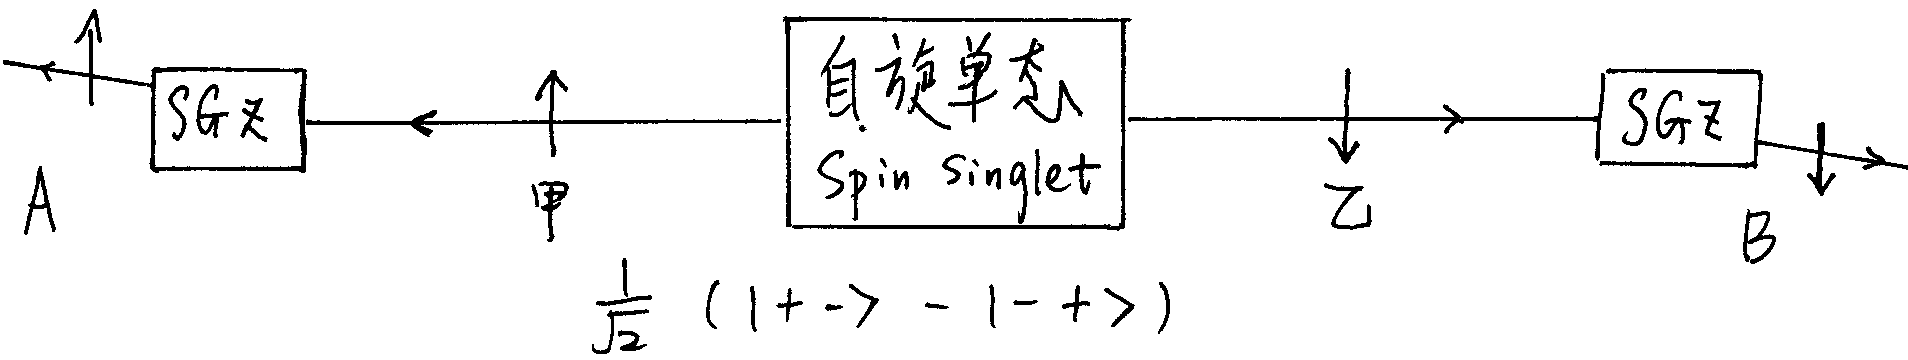
\includegraphics[width=11cm]{DiracNotation/EPRspinsinglet.png}
\caption{自旋相关实验}
\label{default}
\end{center}
\end{figure}

我们在想象中做以下实验:

\begin{enumerate}
\item 

A在左侧不对甲自旋做任何测量,B在右侧对乙自旋测量它在z方向的取值,向上或向下,结果是完全随机的。这里我们没有找到任何物理现实。

\item

A在左侧对甲自旋测量它在z方向的取值,向上或向下,也是随机的;在A完成测量的瞬间,B在右侧对乙自旋也做z方向的测量,在B看来其结果也是随机的,没有任何规律,但如果我们把A和B的测量结果汇总在一起看的话,我们就能发现A和B的测量结果存在着关联,而且是完全的百分百的关联。

比如:只要甲是向上,那么乙就一定是向下;如果甲向下,那乙就一定向上。我们可以把那些使乙确定地“几率为一”地取向上或向下的情形汇总在一起。首先这就符合了爱因斯坦对“物理现实”的定义,这里一定存在一个自旋在z方向上的物理现实。其次量子态比我们设想的要复杂,看起来都叫一个名字,但却可进一步分成很多类,有的自旋向上,有的自旋向下……

\item

我们还可以让A、B都对自旋的x分量进行测量。将得到完全一样的结果。即看起来B对乙自旋x分量的测量是完全随机的,但如果我们把A和B的测量结果拿到一起汇总的话,我们就可以发现对某些测量,B对乙自旋的测量是确定地为向左或向右。Again,按照爱因斯坦对物理现实的定义,自旋的x分量也是“物理现实”的一个要素。

\end{enumerate}

这里要做一个重要的声明,就是我们总是让A先对甲自旋进行测量,而B对乙自旋的测量是在A完成测量的瞬间进行的。如此设计的理由是要保证A在左侧进行的观测——某种扰动——不会影响传播到乙自旋所在的右侧。这样我们可以心安理得的认为B在右侧面对的是同一个量子态。但现在我们所说的量子态必须做集合理解,集合里面有很多假想的乙自旋的态,它们各自又可以分成不同的类,以对应那些可以确定取值的实验。(用物理的术语讲,这个集合就叫系综ensemble\index{Ensemble: 系综})

爱因斯坦这里用到了“定域原则”,即对空间分离的两个系统甲和乙,乙的任何变化不是对甲操作的结果。

如果坚持“定域原则”的话,$S_x$和$S_z$就可以同时是物理现实了,原则上我们可以给系综里的每个自旋指定一个$S_x$的取值,同时一个$S_z$的取值,但我们的量子力学——海森堡、薛定谔和狄拉克的量子力学——无法提供这个信息,在此意义下我们说量子力学是不完备的。

爱因斯坦是这样定义一个物理理论的完备性的:“物理现实的每个要素在物理学理论中都必须有它的对应部分。”

爱因斯坦并不认为量子力学是错的,但他认为量子力学是不完备的,即潜在地还存在着一个升级的版本可以使每个“物理现实”的要素都在理论中有对应,在我们现在的例子下就是$S_x$和$S_z$。

爱因斯坦这里其实是要做一个选择,即在“定域原则”和“不确定原理”之间选择。坚持了“定域原则”,就意味着我们构造了一个$S_x$和$S_z$都要取确定值的例子,这就必须放弃“不确定原理”。

放弃“定域原则”,意味着A在左侧的测量动作会在瞬间对远在右侧的乙自旋进行筛选,即瞬间B所面对的乙自旋的态就发生变化了。我们仍可按海森堡-薛定谔-狄拉克的量子力学对它进行处理,投影到基矢上,并计算几率幅。

放弃“定域原则”并不意味着违反相对论,因为B仅在它的局域进行测量,无法同时知道A对甲自旋的测量结果,所以不论有没有百分百的自旋相关,在B看来它测得的结果都是完全随机的结果,没有任何意义。换句话说我们无法利用纠缠态进行通讯,所以也谈不上违反相对论。

仅仅如此我们是无法判断孰是孰非的。因为爱因斯坦及后来隐变量理论的主张者都没提出替代性的量子理论,所以很难构造实验去进行判定。

\subsubsection{贝尔不等式}

我们同意无法同时确定$S_x$和$S_z$,但假设有很多自旋1/2,我们把$S_z$和$S_x$的取值同时赋予这些自旋,并对它们进行分类,比如我们有(z+,x-),这意味着如果我们对这类自旋测量$S_z$的话,我们将确定地得到向上;我们也可以选择测量$S_x$,确定地得到向下。除了(z+,x-),我们还有相同数量的自旋属于(z+,x+)类。假如我们对筛选出来的$z+$自旋测量$S_x$,50\%的可能性得到$x+$,另外50\%的可能性得到$x-$。

考虑自旋单态(总自旋为0的态),假设自旋可以用(z+,x-)这样的记号进行分类的话,那么(z-,x+)和(z+,x-)就构成一对。总共有四种可能性:

\begin{description}
\item[类型 I:] 

甲(z+,x-);乙(z-,x+)

\item[类型 II:] 

甲(z+,x+);乙(z-,x-)

\item[类型 III:]

甲(z-,x+);乙(z+,x-)

\item[类型 IV:]

甲(z-,x-);乙(z+,x+)

\end{description}

这里对左侧的甲自旋,假如属于第I种类型,A可以对甲测量$S_z$,也可以测量$S_x$,但这些动作都不会改变右侧的乙自旋(z-,x+),这就构造了一个符合爱因斯坦“定域原则”的方案。

进一步讨论,假如A先对甲测量$S_z$,假设结果是向上,这筛选出类型I和类型II,但这个测量动作之后甲和乙就不再是自旋单态了。如果我们再继续对甲测量$S_x$,对乙也测$S_x$,它们的测量结果将失去关联。

在此基础上我们可以讨论贝尔不等式(Bell's inequality)\index{Bell's inequality: 贝尔不等式}。贝尔不等式是贝尔在1964年提出来的,他构造了一个可以区分正统量子力学和符合“定域原则”替代版本量子力学的实验判据。

\begin{figure}[htbp]
\begin{center}
\includegraphics[width=6cm]{IdenticalParticles/john_s_bell.gif}
\caption{贝尔(1928--1990)}
%\label{default}
\end{center}
\end{figure}


其实没有替代版本的量子力学,需要做的是把“定域原则”以某种方式考虑进去。

考虑三个互相不正交的方向:a,b和c。我们可以沿a,b或c的方向测量自旋。然后假设有甲、乙两个自旋,甲向左飞,乙向右飞。

甲和乙构成自旋单态,这意味着如果我们可以用(a-,b+,c+)对甲进行标记的话,那么与甲对应的乙就只能是(a+,b-,c-)。

甲、乙构成的自旋单态可以分为如下八类,每一类的数字用$N_i$表示:

\begin{description}
\item[$N_1$:] 

甲(a+,b+,c+);乙(a-,b-,c-)

\item[$N_2$:]

甲(a+,b+,c-);乙(a-,b-,c+)

\item[$N_3$:]

甲(a+,b-,c+);乙(a-,b+,c-)

\item[$N_4$:]

甲(a+,b-,c-);乙(a-,b+,c+)

\item[$N_5$:]

甲(a-,b+,c+);乙(a+,b-,c-)

\item[$N_6$:]

甲(a-,b+,c-);乙(a+,b-,c+)

\item[$N_7$:]

甲(a-,b-,c+);乙(a+,b+,c-)

\item[$N_8$:]

甲(a-,b-,c-);乙(a+,b+,c+)

\end{description}

这里所有的N都是非负的,我们可以构造如下不等式:

\begin{equation}
N_3 + N_4 \le N_2 + N_4 + N_3 + N_7
\end{equation}

假设我们做这样的实验:A对甲自旋进行测量,让甲通过a方向的非均匀磁场,得到的结果是向上;然后B对乙自旋进行测量,让乙通过b方向的非均匀磁场,假设得到的结果也是向上。如此关联的测量结果对应的数目是:

\begin{equation}
N_3 + N_4
\end{equation}

我们把这个类型记为(a+,b+),得到这个结果的几率是:

\begin{equation}
P(a+, b+) = \frac{N_3 + N_4}{ \sum\limits_i N_i}
\end{equation}

类似地,A对甲自旋进行测量,让甲通过a方向的非均匀磁场,得到的结果是向上;然后B对乙自旋进行测量,让乙通过c方向的非均匀磁场,假设得到的结果也是向上。我们把这个类型记为(a+,c+),对应的几率是:

\begin{equation}
P(a+, c+) = \frac{N_2 + N_4}{ \sum\limits_i N_i}
\end{equation}

还有(c+,b+),对应的几率是:

\begin{equation}
P(c+, b+) = \frac{N_3 + N_4}{ \sum\limits_i N_i}
\end{equation}

这样我们得到一个关于几率的不等式:

\begin{equation}
P(a+, b+) \le P(a+, c+) + P(c+, b+)
\end{equation}

以上是考虑了“定域原则”后的一个不等式。正统量子力学不考虑“定域原则”,但我们可以利用投影直接把以上几率都计算出来。

以a方向为参照,自旋单态可表示为(总自旋为0,同时总自旋在a方向上的分量为0):

\begin{equation}
\left| spin-singlet \right\rangle = \frac{1}{\sqrt{2}}\left( \left|{a+, a- }  \right\rangle  - \left|{a-, a+ }  \right\rangle \right)
\end{equation}

首先我们计算$P(a+, b+)$,a+是对自旋甲而言的,自旋乙就应处于a-的状态,我们需要算的就是一个a-态下的自旋向b+方向投影:

\begin{equation}
\left\langle {b+} | {a-} \right\rangle = \frac{1}{\sqrt{2}} \cos \frac{\pi - \theta_{ab}}{2} 
\end{equation}

这里$\theta_{ab}$指的是方向a和方向b之间的夹角。

\begin{equation}
P(a+, b+) = \left| {\left\langle {b+} | {a-} \right\rangle} \right|^2 = \frac{1}{2} \sin^2 \frac{\theta_{ab}}{2}
\end{equation}

假如正统量子力学也符合贝尔不等式的话,我们应该有:

\begin{equation}
\sin^2 \frac{\theta_{ab}}{2} \le \sin^2 \frac{\theta_{ac}}{2} + \sin^2 \frac{\theta_{cb}}{2}
\end{equation}

我们可以举一个特例来说明贝尔不等式是被违背的,假设a、b和c都在一个平面内,$\theta_{ab} = 2 \theta$,c正好在a和b的中间,$\theta_{ac} = \theta_{cb} = \theta$。考虑$\theta$的取值范围是0到$\frac{\pi}{2}$,我们可以做个表来说明:

%%%%

\begin{table}[htdp]
\caption{量子力学的计算与贝尔不等式不符}
\begin{center}
\begin{tabular}{|c|c|c|}
\hline
$\theta$ &  $\sin^2 \frac{\theta_{ab}}{2}$  & $\sin^2 \frac{\theta_{ac}}{2} + \sin^2 \frac{\theta_{cb}}{2} $ \\
\hline
$\frac{\pi}{20}$ & 0.024  & 0.012  \\
$\frac{\pi}{10}$ & 0.095  & 0.049  \\
$\frac{3\pi}{20}$ & 0.206  & 0.109  \\
$\frac{\pi}{5}$ & 0.345  & 0.191  \\
$\frac{\pi}{4}$ & 0.5  & 0.293  \\
$\frac{3\pi}{10}$ & 0.654  & 0.412  \\
$\frac{7\pi}{20}$ & 0.793  & 0.546  \\
$\frac{2\pi}{5}$ & 0.904  & 0.69  \\
$\frac{9\pi}{20}$ & 0.975  & 0.843  \\
\hline
\end{tabular}
\end{center}
\label{default}
\end{table}%



%%%%

正统量子力学做出了与符合“定域原则”替代理论完全不同的预言。

这样,我们就可以利用实验去验证爱因斯坦的观点了。

迄今为止的实验都表明贝尔不等式被违反了\footnote{比如最近的一项研究:Testing Bell's Inequality with Cosmic Photons: Closing the Setting-Independence Loophole, \url{http://arxiv.org/abs/1310.3288}},在这个意义下我们说量子力学是个“非定域”的理论,对一个纠缠态,某个局部的测量会影响空间分离的另一个局部的状况,这是一种超越距离的瞬时的量子态的坍缩。

那么我们可以通过这种超越距离的瞬时的量子态的改变传递信息吗?比如我们把A、B测量结果100\%相关的情形看做是编码1,而把A、B测量结果一点都不相关的情形定义为编码0,这种方案会奏效吗?正像我们前面讨论过的,B在他的局域,总是面对一组完全随机的测量结果,除非同时他能有A的测量结果并汇总为表格,否则他是没法判断A、B的测量结果是否存在关联的。那么A如何把她的测量结果瞬时传递给B呢?除了打电话可能就没有别的办法了\footnote{写这段的时候,正好在微博上看到一个“笑话”,@灰鸽子银水:“量子纠缠态的超距通信时时被人说起。常有的误解是,一对纠缠态的量子,一个状态发生改变,另一个立即改变——这是超越光速的——用我最喜欢的类比来说,这种改变就像是你在中国的妹妹生了个小孩,远在巴黎的你立即在同时成为了舅舅。你称谓的改变同样是超光速的,但需要一个来自你妹妹的电话才会知道。”}。

这就相当于是在加密传输信息,解密需要的密码本必须预先放在B的手上,他才能解读,但很可惜解密用的密码本不是预先生成的,它是伴随着A对甲自旋的测量临时生成的,A没办法把密码本送过去,B就没法解读他的测量结果中所蕴涵的信息。

~

虽然爱因斯坦在这个问题上判断错误,但我们不能因此就小觑(undervalue)了爱因斯坦的贡献,一个伟大物理学家的错误理论往往比一个平庸物理学家的正确理论对学科的贡献大的多得多。(这意味着在物理学中追求新颖比追求正确更有价值。)

阅读爱因斯坦1935年的论文,我们能够感受到爱因斯坦强健的物理思维,即把哲学的立场——对“物理现实”的坚持——翻译为物理的选择——保留“定域原则”,还是保留“不确定原理”——进而挑战量子理论已经完备的正统观点。

爱因斯坦的这个工作也被看做是今天热门的量子信息学的奠基工作,这篇论文在物理评论网站上显示已经被引用了4249次,而获得了诺贝尔奖的康普顿散射的论文也才仅仅被引用了210次。

\subsection*{练习}

\begin{enumerate}

\item

考虑两个自旋1/2组成的系统,处在态

\begin{equation*}
\left| \alpha \right\rangle = a \left| ++ \right\rangle + b \left| +- \right\rangle + c \left| -+ \right\rangle  + d \left| -- \right\rangle
\end{equation*}

这里态$\left| \alpha \right\rangle $是归一的,即$|a|^2 + |b|^2 + |c|^2 + |d|^2 = 1$。针对这个态测量物理量$S^2$,这里$S$表示总自旋算符,$S = S_1 + S_2$。求:

\begin{enumerate}
\item 

力学量$S^2$的可能测量值是多少?

\item

对每个测量值,它们的概率是多少?(用$a, b, c, d$表示)

\end{enumerate}

\item

$n$是沿空间某方向上的单位向量,它与$z$轴的夹角是$\theta$,它在$x-y$平面上的投影与$x$轴的夹角是$\phi$。

对自旋1/2,求$S \cdot n$的本征值问题。

\begin{figure}[htbp]
\begin{center}
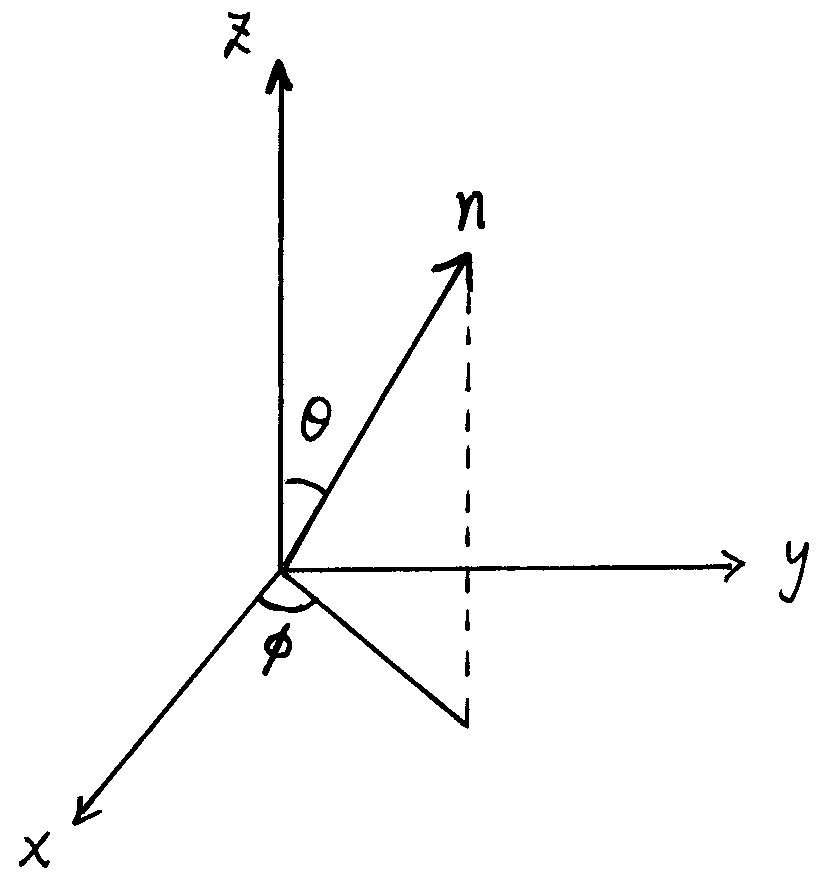
\includegraphics[width=6cm]{DiracNotation/sigma_n.png}
\caption{$n$与$z$轴的夹角是$\theta$,$n$在$x-y$平面上的投影与$x$轴的夹角是$\phi$。}
%\label{default}
\end{center}
\end{figure}


\end{enumerate}




